% !TEX root = ../notes_template.tex
\chapter*{Preface}
\addcontentsline{toc}{chapter}{Preface}

\lipsum % dummy text - remove from real document

\section{Features of this template}

\begin{itemize}
    \item crossref: different styles of clickable definitions and theorems
    \begin{itemize}
        \item nameref:
            \nameref{def:gaussian_distribution}

        \item autoref:
            \autoref{def:gaussian_distribution}

        \item cref:
            \cref{def:gaussian_distribution}

        \item hyperref:
            \hyperref[def:gaussian_distribution]{Gaussian}
    \end{itemize}

    \item toc: list of theorems, definitions
    \item bib: titles of reference is linked to the publisher webpage 
        \cite{kitaev2002classical}
        \cite{childsUniversalComputationQuantum2009}
    \item index
    \myindex{index} 
    \item glossary:
    \gls{real_number},
    \gls{natural_number},
    \gls{complex_number},
    \gls{svm},
    \gls{v}
    \begin{itemize}
        \item glossary package
        \item glossary-extra package and bib2gls
    \end{itemize}
\end{itemize}

\subsection{Cross reference}

\begin{figure}[!ht]
    \centering
    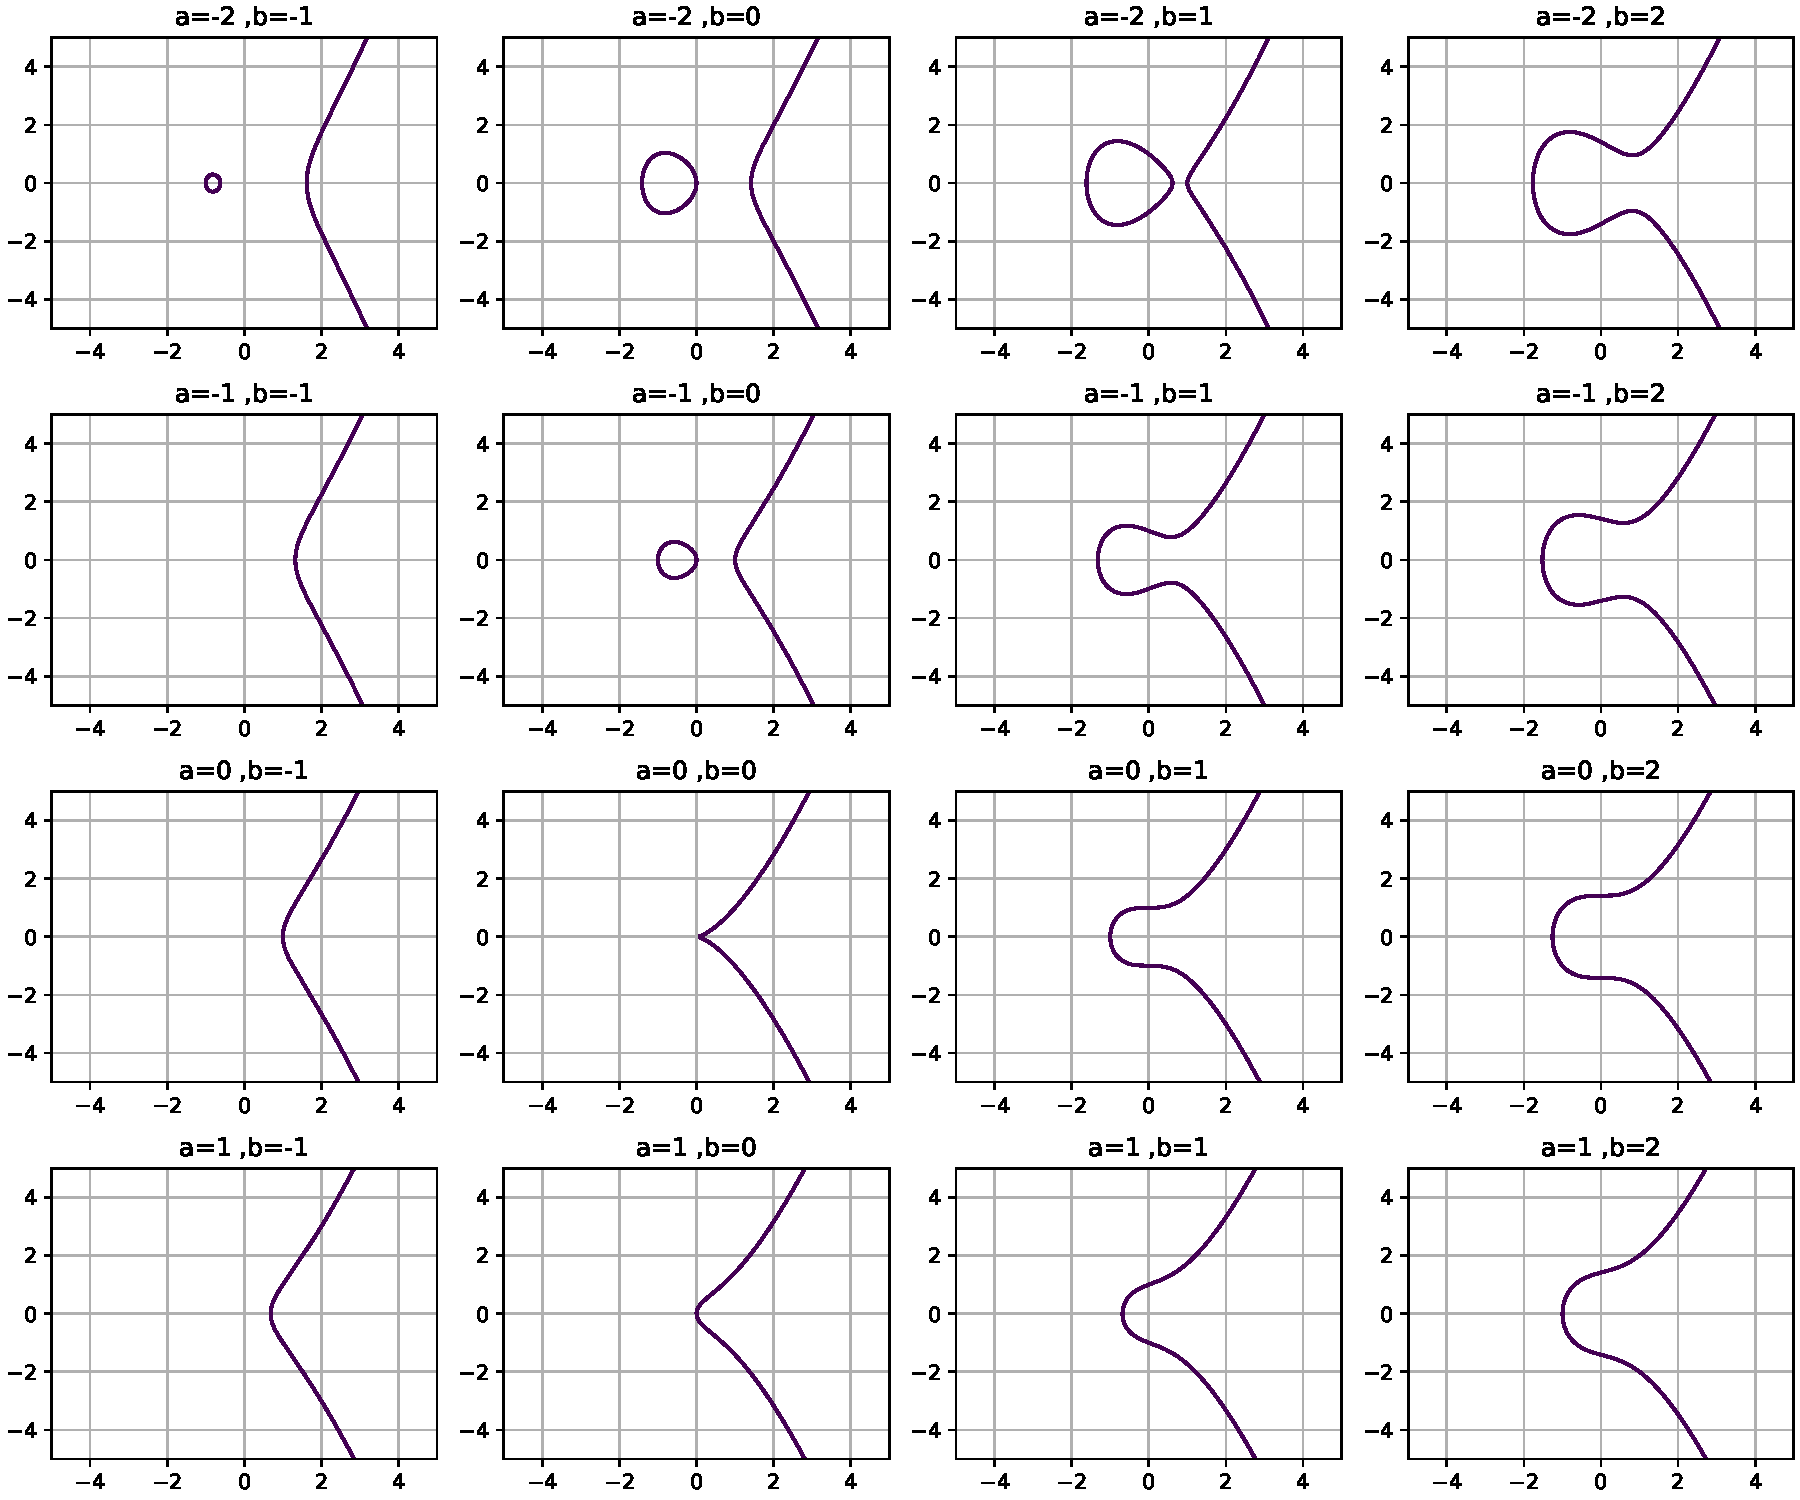
\includegraphics[width=1\linewidth]{./figure/elliptic_curves.pdf}
    \caption{Elliptic curves}
\end{figure}